\documentclass[main.tex]{subfiles}

\begin{document}
	
\section{Spracovanie údajov o vlakových sieťach}

Pre každú krajinu sme získali dva typy súborov. Prvý typ obsahoval údaje o jednotlivých staniciach v danej krajine, teda názvy staníc a ich zemepisné šírky a dĺžky. Druhý typ obsahoval údaje o prepojeniach medzi stanicami, teda dvojice bodov vyjadrené pomocou zemepisných šírok a dĺžok.

Bohužiaľ, tieto typy údajov nebolo možné priamo namapovať na seba kvôli nekonzistenciám v údajoch. Preto sme použili heuristický prístup, pri ktorom sme pre každé spojenie určili začiatočnú a konečnú stanicu ako tie stanice z datasetu, ktoré sú najbližšie k začiatočnému a konečnému bodu spojenia. Týmto spôsobom sa nám podarilo vytvoriť graf reprezentujúci železničné siete pomocou knižnice \texttt{NetworkX}. Následne, pre doplnenie údajov, sme do grafu pridali váhy hrán reprezentujúce vzdušnú vzdialenosť medzi stanicami, keďže naše údaje neposkytovali presné vzdialenosti medzi prepojenými stanicami.

\begin{figure}
\centerline{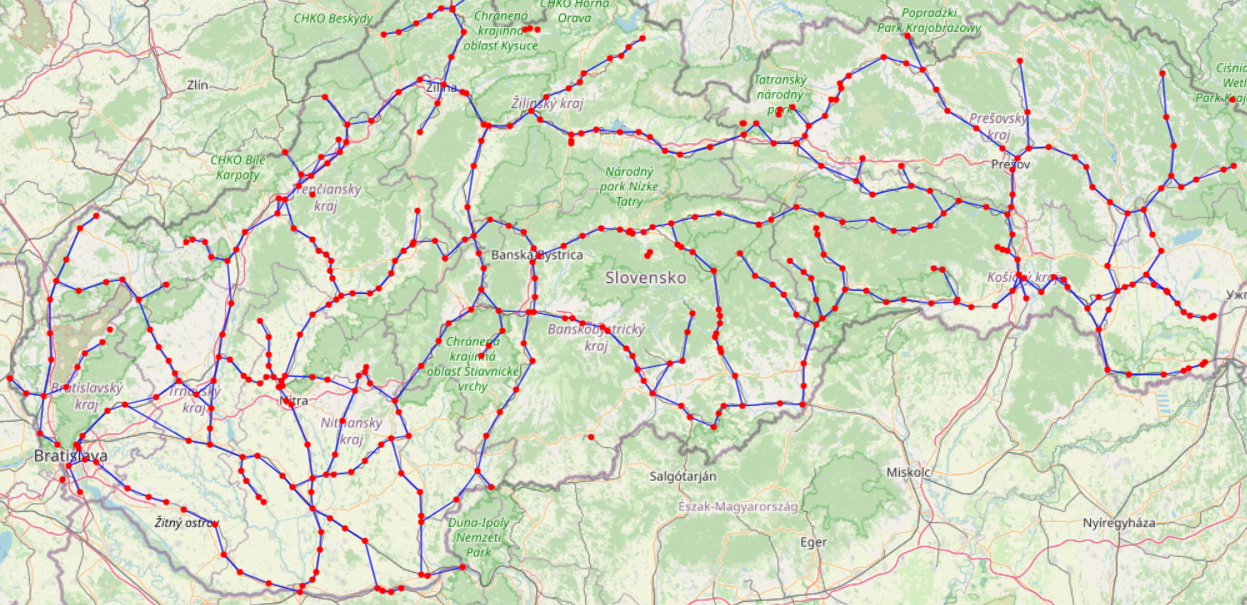
\includegraphics[width=1\textwidth]{images/first_attempt_slovakia.png}}
\caption{Prvotný pohľad na našu reprezentáciu slovenskej železničnej siete}
\label{obr:Slovakia_first}
\end{figure}

\begin{figure}
\centerline{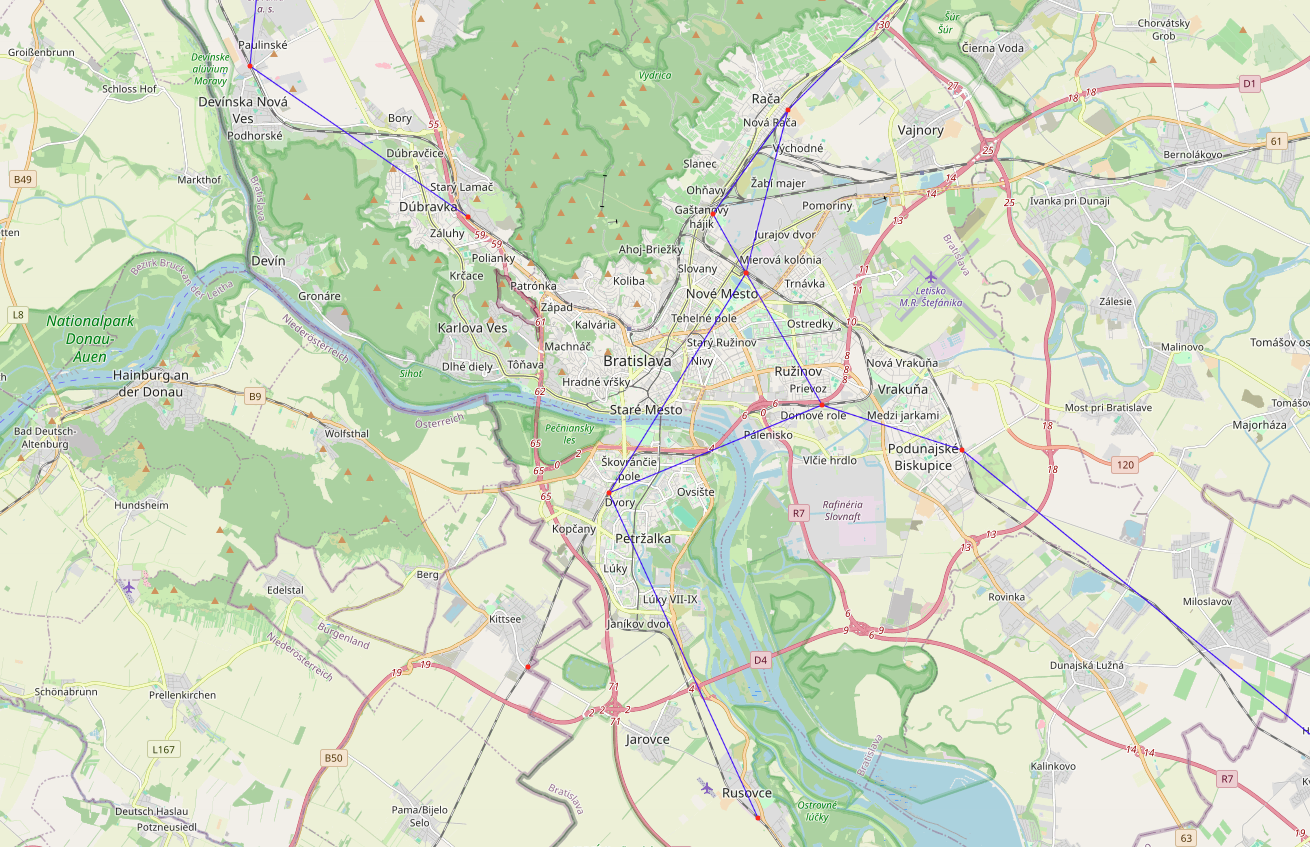
\includegraphics[width=1\textwidth]{images/first_attempt_bratislava.png}}
\caption{Prvotný pohľad na reprezentáciu slovenskej železničnej siete v okolí Bratislavy}
\label{obr:Bratislava_first}
\end{figure}

Z prvotného pohľadu na našu reprezentáciu slovenskej železničnej siete (obrázok \ref{obr:Slovakia_first}) môžeme povedať, že zachytáva reálnu sieť relatívne dobre, avšak s niekoľkými nedostatkami. Napríklad stanica vo Veľkom Krtíši nie je prepojená so žiadnou inou stanicou. Dôvodom je, že v realite je prepojená s Lučencom, ale traťou prechádzajúcou cez Maďarsko. Práve takéto hrany, ktoré prechádzajú cez zahraničné územie, v našej sieti chýbajú. Podobne, pri bližšom pohľade na oblasť Bratislavy (obrázok \ref{obr:Bratislava_first}), sme zistili, že nie je zahrnutá Bratislava hlavná stanica a tiež nie je prepojená trať smerom na Záhorie. Na základe týchto zistení sme manuálne doplnili niekoľko hrán a staníc do grafu slovenskej železničnej siete.

\begin{figure}
\centerline{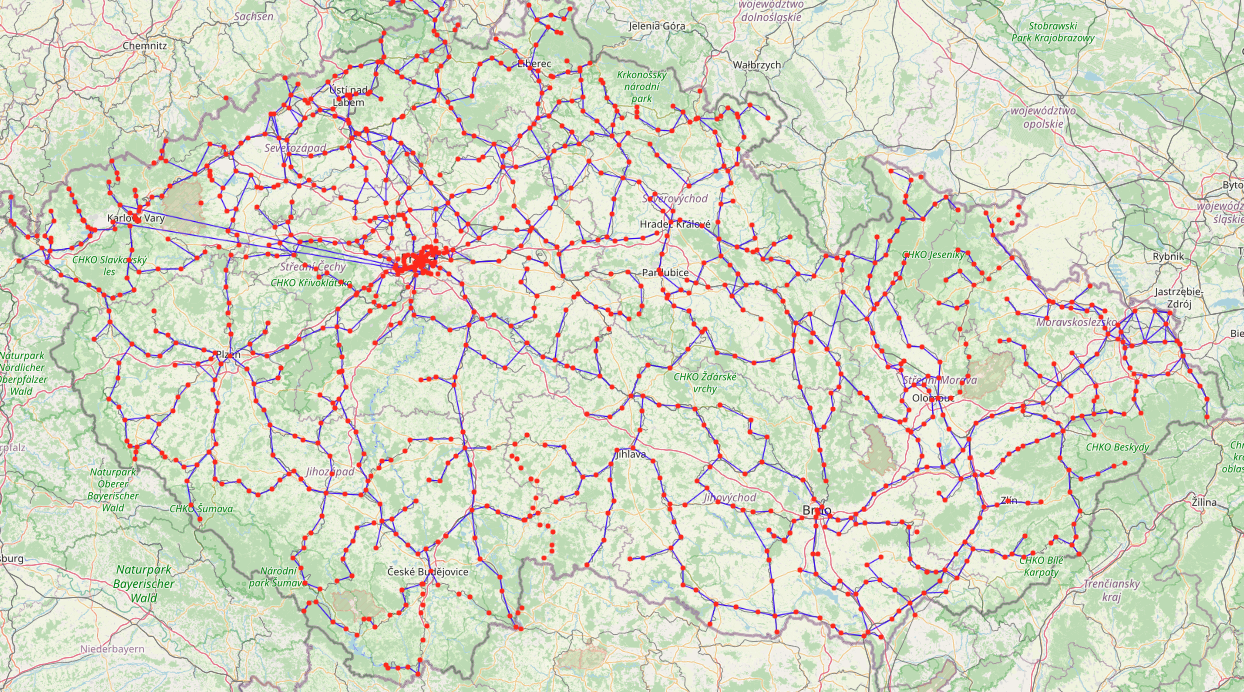
\includegraphics[width=1\textwidth]{images/first_attempt_czechia.png}}
\caption{Prvotný pohľad na našu reprezentáciu českej železničnej siete}
\label{obr:Czechia_first}
\end{figure}

\begin{figure}
\centerline{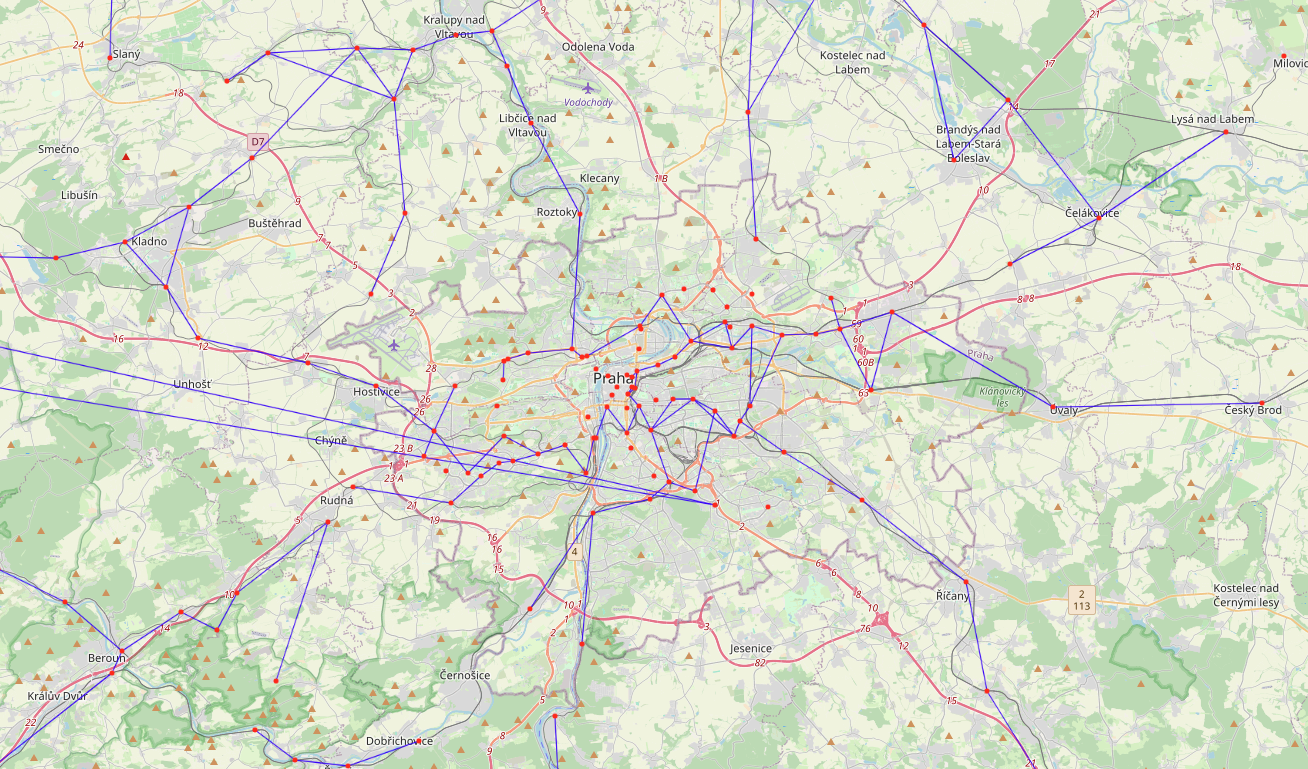
\includegraphics[width=1\textwidth]{images/first_attempt_praha.png}}
\caption{Prvotný pohľad na našu reprezentáciu českej železničnej siete v okolí Prahy}
\label{obr:Praha_first}
\end{figure}

Pre českú železničnú sieť, ktorá je rozsiahlejšia, vzniklo výrazne viac nekonzistencií s realitou. Prvým problémom, ktorý sme identifikovali, bolo, že sa do nášho datasetu dostali zastávky pražského metra (obrázok \ref{obr:Praha_first}). Rozhodli sme sa ich nepoužiť, keďže metro nepatrí priamo k vlakovej doprave, ale skôr k mestskej hromadnej doprave. Toto však narušilo sieť v okolí Prahy, a preto sme museli manuálne pridať množstvo hrán a tiež niekoľko staníc. Okrem toho, na obrázku \ref{obr:Czechia_first} môžeme vidieť viacero staníc, ktoré nie sú prepojené so žiadnymi inými stanicami, napríklad v okolí Českých Budějovíc. Pri bližšom pohľade sme však zistili, že v realite existujú spojenia pre tieto stanice. Takýchto nepravidelných výpadkov bolo v sieti pomerne veľa. Keďže sme nenašli lepšie riešenie, rozhodli sme sa manuálne doplniť väčšinu siete, aby sme zabezpečili, že naša reprezentácia je čo najbližšie k realite. Nakoniec sme do českej siete pridali viac ako 170 spojení, odstránili 59 staníc a tiež odstránili niekoľko neexistujúcich spojení.




% Po finálnych úpravách mala siet Slovenska 426 staníc a 449 spojení medzi danými stanicami. Sieť Česka za to mala skoro tri krát viac staníc a spojení, presnejšie 1146 staníc a 1262 spojení. V obrázku \ref{obr:Combined_final} si čitateľ môže pozrieť mapu na ktorej sú zobrazené obidve siete naraz. 

% \begin{figure}[H]
% \centerline{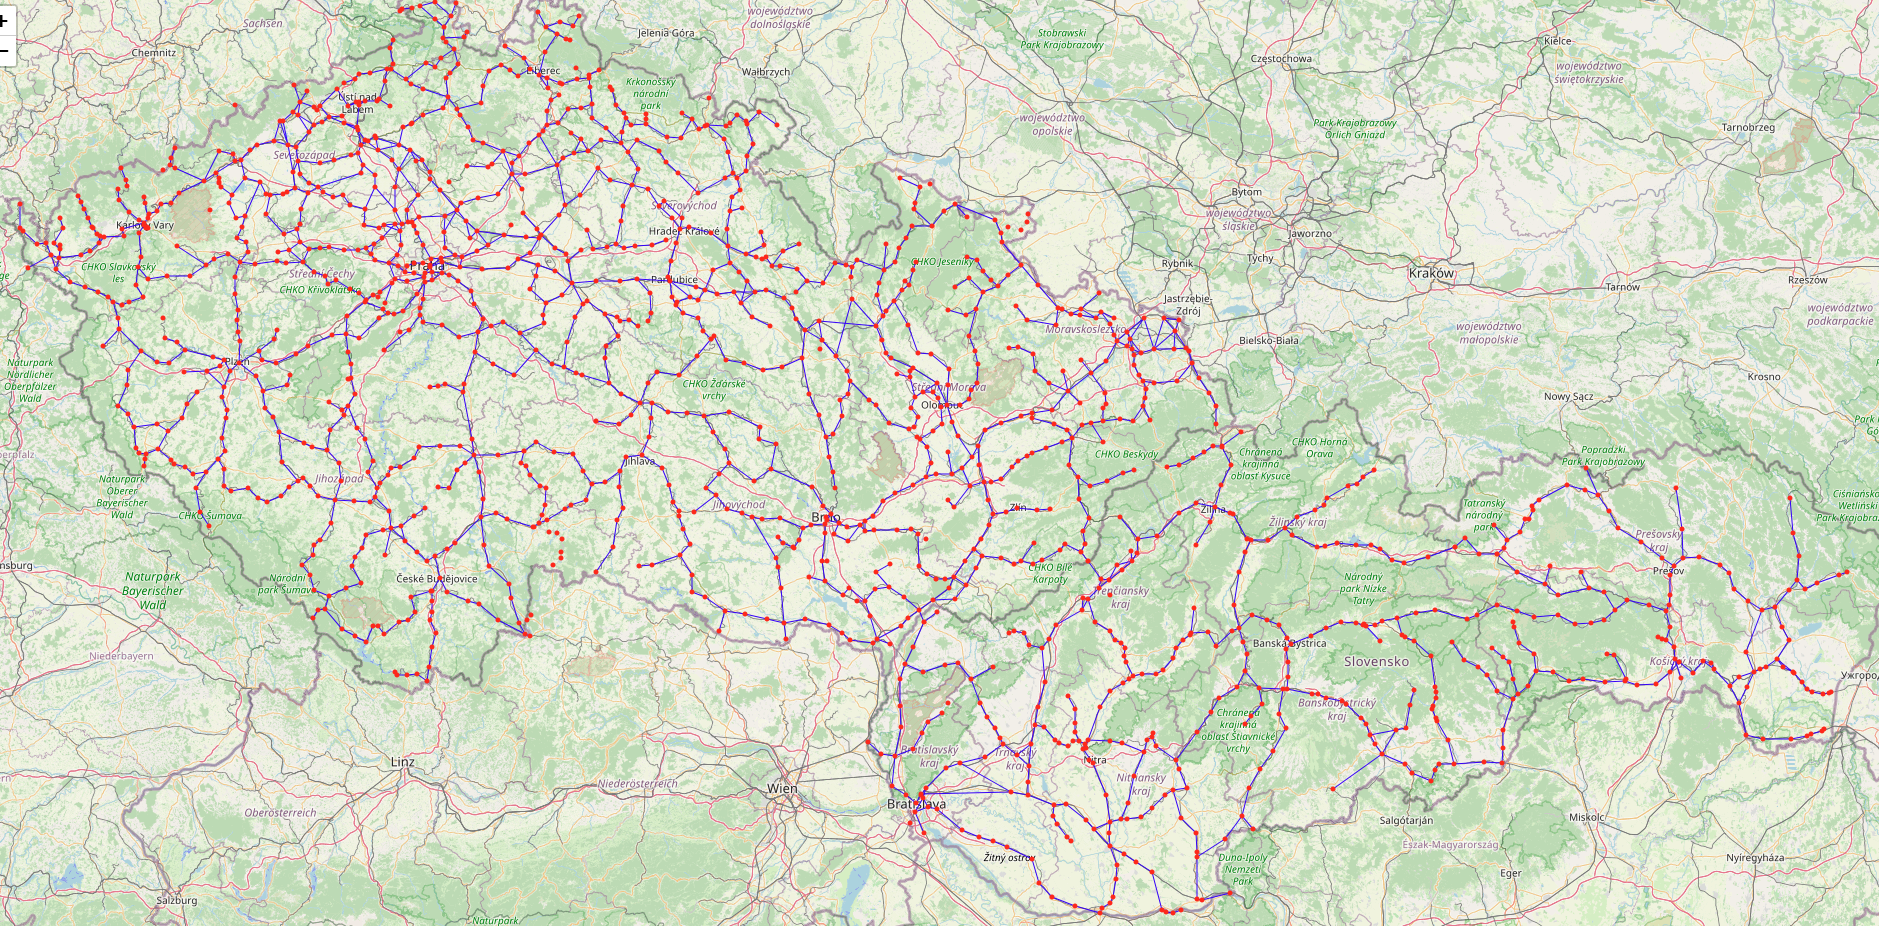
\includegraphics[width=1\textwidth]{images/combined_map_final.png}}
% \caption{Finálny grafy našich reprezentácií Ćeskej a Slovenskej železničnej siete}
% \label{obr:Combined_final}
% \end{figure}
\end{document}